\section{Methods}

\subsection{Ploidy and breeding system data}

%B: IMO: The data subsection would be better organized with parts, (1) ploidy, (2) breeding system, (3) tree, (4) models, (5) model selection and statistical inference.

Chromosome number data were obtained for all Solanaceae taxa in the Chromosome Counts Database \citep[CCDB;][]{rice_2015}, and the ca.~14,000 records were curated semi-automatically using the CCDBcurator R package \citep{rivero_2019}.
CCDB contains records from original sources that have multiple complex symbol patterns denoting multivalence, or irregularites of chromosome counts.
After a first full round of curation via CCDBcurator, we contrasted results by hand and corrected chromosomes where CCDBcurator's output was not able to adequately correct records.
Our hand-curated records were also contrasted against the ploidy dataset from \citet{robertson_2011} and against ploidy data in the C-value DNA dataset from \citet{bennett_2005}.
%B: perhaps "cleaned" should be explained, unless it's hard to identically repeat as-is. R- I added more (it only took 4months to hand-curate 14,000 entries
By comparing three different sources of information, we were able to code taxa as diploid (D) or polyploid (P).
For the majority of species, ploidy was assigned according to information from the original publications included in the  C-value DNA dataset \citep{bennett_2005}.
For taxa without ploidy information but with information about chromosome number, we assigned ploidy based on the multiplicity of chromosomes within the genus or based on SI/SC classification.
For example, \textit{Solanum betaceum} did not have information about ploidy level but it has 24 chromosomes, so since $x=12$ is the base chromosome number of the \textit{Solanum} genus \citep{olmstead_2007}, we assigned \textit{S.~betaceum} as diploid. 
Additionally, because of the absence of SI polyploids (discussed further below), species known to be SI could be scored as diploid.
Species with more than one ploidy level were assigned the most frequent ploidy level recorded or the smallest ploidy in case of frequency ties.

Breeding system was scored as self-incompatible (I) or self-compatible (C) based on results curated from the literature and  original experimental crosses \citep[as compiled in][]{igic_2006, goldberg_2010, robertson_2011, goldberg_2012}.
Many species could unambiguously be coded as either I or C \citep{raduski_2012}.
Following previous work, we coded as I any species with a functional SI system, even if SC or dioecy was also reported.
Dioecious species without functional SI were coded as C.
% E: I am trying to stick with I/C when talking about the state values, but using SI/SC when talking about the meaning of the trait (because this what people use normally). 
%R- Okay- I was getting confused as well thanks for clarifying

The Supplementary Information contains citations for the numerous original data sources. % todo: say how many refs?
Resolution of taxonomic synonymy followed the conventions provided in Solanaceae Source \citep{solsource}. 
Hybrids and cultivars were excluded because ploidy and breeding system can be affected by artificial selection during domestication.
Following the reasoning outlined in \citet{robertson_2011}, we examined closely the few species for which the merged ploidy and breeding system data indicated the presence of self-incompatible polyploids.
Although SI populations frequently contain some SC individuals, and diploid populations frequently contain some polyploid individuals, in no case did we find a convincing case of a naturally occurring SI and polyploid population.
The single instance of an SI polyploid individual appears to be an allopentaploid hybrid of \textit{Solanum oplocense} Hawkes x \textit{Solanum gourlayii} Hawkes, reported by \citet{camadro_1981}.
Under exceedingly rare circumstances, it is possible for polyploids containing multiple copies of S-loci to remain SI, so long as they express a single allele at the S-locus \citep[discussed in][]{robertson_2011}.
Because of the resulting absence of SI and polyploid populations, as well as the linked functional explanation for disabling of gametophytic self-incompatibility systems with non-self recognition, following whole genome duplication \citep[reviewed in][]{ramsey_1998,stone_2002}, we consider only three observed character states: self-incompatible diploids (ID), self-compatible diploids (CD), and polyploids which are always self-compatible (CP).
%B: I added the non-self recognition bit, because in Prunus, heteroallelic pollen may not cause SC.

Matching our character state data to the largest time-calibrated phylogeny of Solanaceae \citep{sarkinen_2013} yielded 595 species with ploidy and/or breeding system information on the tree.
Binary or three-state classification of ploidy and breeding system for the 595 taxa is summarized in \cref{figure:stateclassifications}.
We retained all of these species in each of the analyses below because pruning away tips lacking breeding system in the ploidy-only analyses (and vice versa) would discard data that could inform the diversification models.
A total of 405 taxa without any information about breeding system or polyploidy were excluded.
%Tips without trait data might not improve point estimation of diversification parameters while increasing uncertainty in the estimates of trait linked diversification
% R-This is very important but I have removed it because I think it is a full on paper by its own
Including this many more species would have prohibitively slowed our analyses, especially those implementing the most complex models.

% D/P ploidy model
% D/P+A/B ploidy hidden state model
% I/C breeding system model
% I/C+A/B breeding system and hidden state model
% ID/CD/CP ploidy and breeding system model
% ID/CD/CP+A/B ploidy, breeding system, and hidden state model

\subsection{Models for ploidy and diversification}

In order to investigate the association between ploidy level and diversification, we first defined a binary state speciation and extinction model (BiSSE, \citealt{maddison_2007}) in which taxa were classified as diploid (D) or polyploid (P).
We call this the D/P ploidy model.
The model parameters are speciation rates ($\lambda_D$, $\lambda_P$) and extinction rates ($\mu_D$, $\mu_P$) for each state, and a rate of transition from D to P ($\rho$).

% E: I moved r and nu to later, under statistical inference.  It made it seem like there were too many parameters here.
% I also removed italics around the model names because we don't actually use those names later on (more just the state codes).

Our second model addressed diversification due to ploidy differences while also parsing out the heterogeneity of diversification rates due a possible unobserved trait.
Diversification rate differences explained by some trait other than ploidy were accommodated by adding a hidden state (HiSSE model; \citealt{beaulieu_2016}). %B: inserted "(trait)", because that seems to be the goal - a biological explanation?
% R- Now this is mentioned in the intro so that  makes it easier to write here
In this model, each of the observed diploid and polyploid states were subdivided by a binary hidden trait with states $A$ and $B$.
This model was called the D/P+A/B ploidy and hidden state model. 
Model parameters include speciation rates ($\lambda_{D_A},\ \lambda_{D_B},\ \lambda_{P_A},\ \lambda_{P_B}$) and extinction rates ($\mu_{D_A},\ \mu_{D_B},\ \mu_{P_A},\ \mu_{P_B}$) for each subdivided state.
The polyploidization rate is again represented by $\rho$, and the rates of transition between hidden states are symmetrical with parameter $\alpha$.

\subsection{Models for breeding system and diversification}

To assess the effects of breeding system in the diversification process, we first fit a model in which the states are self-incompatible (I) or self-compatible (C).
This is the same as the analysis of \citet{goldberg_2010}, but with an updated phylogeny \citep{sarkinen_2013}.
We call this BiSSE model the I/C breeding system model. 
It has parameters for state-specific speciation ($\lambda_I,\ \lambda_C$) and extinction ($\mu_I,\ \mu_C$), and for transitions from I to C ($q_{IC}$).

To parse out the effect of breeding system on diversification, while allowing for the possibility of heterogeneous diversification rates unrelated to breeding system, we subdivided each of those states into hidden states $A$ and $B$.
We call this HiSSE model the I/C+A/B breeding system and hidden state model.
It also has parameters for state-specific speciation ($\lambda_{I_A},\ \lambda_{I_B},\ \lambda_{C_A},\ \lambda_{C_B}$) and extinction ($\mu_{I_A},\ \mu_{I_B},\ \mu_{C_A},\ \mu_{C_B}$), for loss of SI ($q_{IC}$), and for transitions between hidden states ($\alpha$).
An I/C+A/B model was used by \citet{freyman_2017} used to study diversification in Onagraceae, but here we restricted the hidden state transitions to be symmetrical. 

Self-incompatibility is homologous in all species in which S-alleles have been cloned and controlled crosses performed.
All species sampled to date possess a non-self recognition, RNase-based gametophytic self-incompatibility \citep[shared even with other euasterid families;][]{ramanauskas_2017}.
Furthermore, species that are distantly related within this family carry closely-related alleles, with deep trans-specific polymorphism at the locus that controls the SI response \citep{ioerger_1990, igic_2006}.
This represents very strong evidence that the $I$ state is ancestral in Solanaceae, and that the SI mechanism was not regained within this family.
Therefore, for all breeding system models, we estimated a transition rate from $I$ to $C$  but not the reverse ($q_{CI}=0$).
% This is an important assumption because ancestral state reconstruction in the models might differ when polyploidy and breeding system are analyzed as independent in the Solanaceae tree.
%
%B: What happens if SC->SI is not fixed? Asking for a friend.  E: Surprisingly, Rosana reports, results are not turned on their head. 
%B: Whew, I was worried. Er, "friend" says thanks. R- Your welcome, by mistake I did that model with reversibility from C to I. I didn't run it for as long as the rest but preliminary ancestral reconstructions seem almost identical when you add that parameter than when you don't. 

\subsection{Models for ploidy, breeding system, and diversification}

Polyploidy and breeding system might influence lineage diversification individually, but these two traits also have complex interactions in Solanaceae species.
Therefore, we considered a multi-state model that investigates the contribution of both traits and the possible transitions between them.
Self-incompatible diploids (ID), self-compatible diploids (CD), and polyploids, which are always self-compatible (CP) were used in a MuSSE model \citep{fitzjohn_2012}.
We did not include a state for self-incompatible polyploids because they are not observed in the data, and  that trait combination state is mechanistically predicted not to occur.
We call this the ID/CD/CP ploidy and breeding system model.
It has six parameters for diversification in each state ($\lambda_{ID},\ \lambda_{CD},\ \lambda_{CP}$ for speciation, $\mu_{ID},\ \mu_{CD},\ \mu_{CP}$ for extinction), and three for transitions between states ($\rho_I,\ \rho_C$ for polyploidization transitions from $ID$ and $CD$ to $CP$, respectively; $q_{IC}$ for loss of self-incompatibility without polyploidization, from $ID$ to $CD$).
The total rate of loss of self-incompatibility, \ie transitions out of $ID$, is $q_{IC} + \rho_I$.
% Diploidization from $CP$ to $ID$ is not allowed because it would represent a simultaneous regain of SI. % E: moved into the diploidization section

The ID/CD/CP model could also suffer from a high type I error, just like a two state BiSSE model. 
We therefore added a hidden trait layer on top of our three-state model \citep[analogous to][]{caetano_2018,  huang_2018}.
We refer to this as the ID/CD/CP+A/B model.
A fully parameterized version of this model would have 26 rate parameters. 
Because our goal was to look for diversification rate differences associated with ploidy and breeding system rather than the specific effects of the hidden states, we fit a simplified version with 15 parameters.
The reduction in parameter space was achieved by fixing the rates for transitions among hidden states to be equal with rate $\alpha$, and fixing the transition rates between observed states to be independent of the hidden state (rates $\rho_I,\ \rho_C,\ \delta,\ q_{IC}$ as defined for the ID/CD/CP model).
There are additionally twelve diversification rate parameters ($\lambda_{ID_A},\ \lambda_{ID_B},\ \lambda_{CD_A},\ \lambda_{CD_B},\ \lambda_{CP_A},\ \lambda_{CP_B},\ \mu_{ID_A},\ \mu_{ID_B},\ \mu_{CD_A},\ \mu_{CD_B},\ \mu_{CP_A},\ \mu_{CP_B}$).
%B: I can't tell, but it seems to me that this 26->16 parameter reduction makes it possible to underestimate the effect of these hidden states.Perhaps this complication is covered in the Discussion section. 
%R- It is possible, but adding all the parameters can also result in an underestimation of the hidden states contribution because it is not enough sample to accurately estimate transitions. In my simulations for diversification-free models, accurately estimating 10 parameters can only be achieved with trees with more than 500 tips. Because of that experience I think 16 parameters is already pushing really the inference machine hard. This happens because the phylogeny is not an independent sample so your ESS is much much smaller and you might end up over-parameterizing.

\subsection{Pathways to polyploidy}

Considering ploidy and breeding system together, there are two evolutionary pathways from SI diploid to SC polyploid \citep{brunet2001, robertson_2011}.
In the one-step pathway, the CP state is produced directly from the ID state when whole genome duplication disables SI.
In the two-step pathway, the CD state is an intermediate: SI is first lost, and later the SC diploid undergoes polyploidization.
We quantify the relative contribution of these pathways to polyploidy in two ways, each using the maximum a posteriori (MAP) estimates of rates from the IC/CD/CP model.

Both of our methods are based on a propagation matrix that describes flow from ID to CP, as in \citet{robertson_2011}.
We insert an artificial division in the CP state, so that one substate contains the CP species that arrived via the one-step pathway and the other substate contains the CP species that arrived via the two-step pathway.
We consider only unidirectional change along each step of the pathway in order to separate them into clear alternatives, and because in this family there is no support for regain of SI, and not strong support for diploidization (see below).
First, we consider only the rates of transitions between these states, placing them in the propogation matrix \myvec{Q}.
The matrix $\myvec{P} = \exp(\myvec{Q} t)$ then provides the probabilities of changing from one state to any other state after time $t$.
Closed-form solutions for the two pathway probabilities are provided in \citet{robertson_2011}.
Our results will differ from those of \citet{robertson_2011} because our transition rate estimates come from a dated phylogeny and a model that allows for state-dependent diversification.
%
Second, we consider not only transitions between states but also diversification within each state.
State-dependent diversification can change the relative contributions of the two pathways.
In particular, if the net diversification rate is small for CD, the two-step pathway will contribute relatively less.
We therefore include the difference between speciation and extinction along the diagonal elements of the propogation matrix.
As before, matrix exponentiation provides the relative chance of changing from one state to any other state after time $t$.
In this case, however, these are not probabilities because diversification changes the number of lineages as time passes.
We can still use their ratios to consider the relative contribution of each pathway, though, analogous to the normalized age structure in a growing population. % R- here a reference would be nice

% "one-step predictions for P_I and P_C over time"
% E & R todo later: for the case with net div, write out the propogation matrix and equations for pathway contributions

\subsection{Diploidization as an exploratory hypothesis}

For the models with ploidy changes, we allowed diploidization by adding a parameter $\delta$ for transitions from P back to D (in the D/P and D/P+A/B models) or from CP back to CD (in the I/C and I/C+A/B models).
We did not allow transitions from CP back to ID because that would include regain of SI.
The models are denoted with $+\delta$ in \cref{table:marginallike}.
Previous modeling approaches \citep{mayrose_2011} have argued against inferring diploidization rates when using ploidy data that comes from classifications based on chromosome number multiplicity or chromosome number change models like chromEvol \citep{mayrose_2010, glick2014, mayrose_2015, freyman_2017}.
These types of classifications do not allow for a ploidy reversion.
Where indicated, the classification of ploidy for the data used in our models was based on chromosome multiplicity at the genus level (see Supplementary Information). % (data available at https://www.github.com/roszenil/solploidy/datasets).
However, the majority of the ploidy classifications were adopted from original studies with alternative sources of information (\eg geographic distribution, genus ploidy distribution) where ploidy was defined by authors that found evidence for it.
Since it is not clear whether diploidization can be detected under alternative ploidy classifications or even classifications based on chromosome number multiplicity at the genus level, we fit models with and without diploidization in order to test  whether the conclusions about diversification are sensitive to including diploidization.
As discussed by \citet{servedio_2014}, the presence or absence of a process can have an exploratory goal.
In our case the diploidization parameter (or its absence, $\delta=0$) in our models is an opportunity to explore an assumption that might be important but that is not the most essential process to understand the interactions among polyploidy, breeding system, and diversification.

\subsection{Statistical inference under the models}

Parameters for each of the ten models described were estimated using RevBayes \citep{hoehna_2016}.
Code for analyses and key results are available at \url{https://github.com/roszenil/solploidy}.
We used the method of \citet{fitzjohn_2009} to account for incomplete sampling in all analyses by setting the probability of sampling a species at the present to $595/3000$ since the Solanaceae family has approximately 3,000 species as estimated by the Solanaceae Source project \citep{solsource}.
For all models, we assumed that speciation and extinction parameters had log-normal prior distributions with means equal to the expected net diversification rate $(\text{number of taxa} / [2 \times \text{root age}])$ and standard deviation $0.5$.
Priors for parameters defining trait changes were assumed to be gamma distributed with parameters $k=0.5$ and $\theta=1$. 
For each model, a Markov chain Monte Carlo \citep[MCMC;][]{metropolis1953equation,Hastings1970} was run for 96 hours in the high-performance computational cluster at the Minnesota Supercomputing Institute, which allowed for 5,000 generations of burn-in and a minimum of 200,000 generations of MCMC for each of the 10 models. %B: the number of models changes here? R-my mistake! fixed it
Convergence and mixing of each MCMC chain was determined by ensuring the effective sample size of each parameter was over 200.

We report posterior distributions for the model parameters, and also for the compound parameters of net diversification ($\lambda - \mu$) and extinction fraction ($\mu / \lambda$) for each state.
Additionally, ancestral states at each node in the phylogeny were sampled jointly during the MCMC analyses.
Ancestral state reconstructions for all models can be found in the Supplementary Information and show the maximum a posteriori of the marginal probability distributions for each of the 594 internal nodes for each of the 10 models. % TODO: add fig refs (or remove the mention of them)

\subsection{Model selection}

We calculated the marginal likelihood for each of the ten models in RevBayes \citep{hoehna_2016}.
Marginal likelihoods were calculated using 50 stepping stone steps under the methodology of \citet{xie_2010}.
Each stepping stone step was found by calculating 500 generations of burn-in followed by a total of 1,000 MCMC steps (\cref{table:marginallike}).
The calculation of each marginal likelihood ran for 24 hours on a high-performance computational cluster.

Using the marginal likelihood values, we calculated thirteen different Bayes factors.
Six compared the models of ploidy against one other (D/P and D/P+A/B, each with or without diploidization), one compared the breeding system models (I/C and I/C+A/B), and six compared the models with both traits (ID/CD/CP and ID/CD/CP+A/B, each with or without diploidization) (\cref{table:bayesfactors}).
%
Other comparisons between these models are not valid because the input data are different under the different state space codings (\cref{figure:stateclassifications}).
In mathematical terms, the D/P, I/C, and ID/CD/CP state spaces are not `lumpable' with respect to one another \citep{tarasov_2019}.
% E: I think this short explanation is clear enough, especially with the figure.  I'm not sure whether the hierarchical concept is exactly applicable here.
%R: Boris in the introduction mentions this possible causal relationship would that be equivalent to say hierarchical?
Each model comparison is reported with a Bayes factor on the natural log scale: the comparison between models $M_0$ and $M_1$ is $BF(M_0,\ M_1) = \ln[ P(\mathbf{X} | M_0) - P(\mathbf{X} | M_1]$.
There is `positive' support for $M_0$ when this value is more than 2, `strong' support when it is more than 6, and `very strong' support when it is more than 10 \citep{kass1995}.

\begin{figure}
\centering
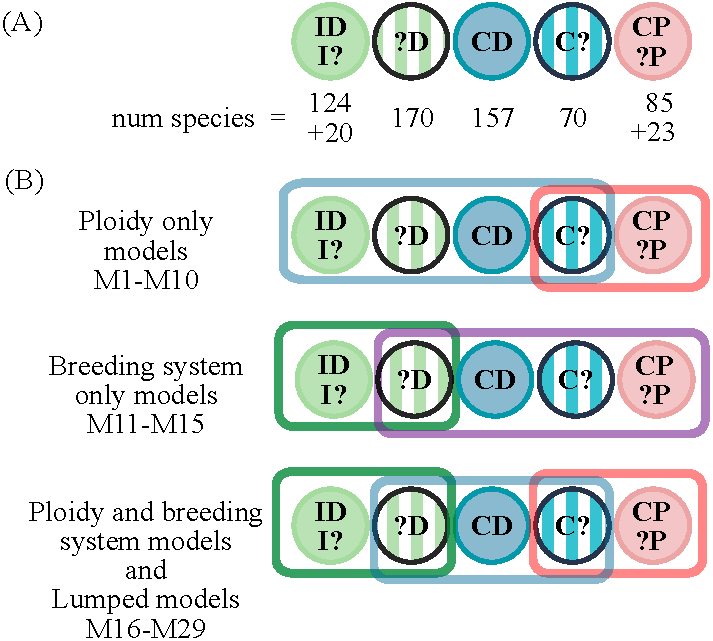
\includegraphics[width=0.5\textwidth]{states.pdf}
\caption{
Character states used for each of the models.
Each species retained on the tree belonged to one of five possible categories, depending on whether ploidy and/or breeding system were known.
The number of species in each is shown under the corresponding circles in the top row. % FIXME: Rosana, what are the numbers for CP and ?P ?
These categories were then grouped in a manner appropriate to the states of each model.
For example, there are 34 species that are self-compatible and of unknown ploidy; these are coded as either $D$ or $P$ in the D/P models (uncertain, or consistent with either state), as $C$ in the I/C models, and as either $CD$ or $CP$ in the ID/CD/CP models.
In all cases, species were coded as either $A$ or $B$ in the hidden state models.
The models depicted in the different rows use state spaces that are not comparable with one another.
For example, we cannot test whether the D/P model fits better than the I/C model because they use states that are not the same and are not `lumpable' \citep{tarasov_2019}.
%B: Hmmm. The presentation is economical, true, and I think it is retrospectively clear, and valuable, now that I've been thinking about the paper for a while. But it will be very difficult as a source of clarity for someone reading the paper the first time. The top graphical layout also implicitly communicates the idea that all "I" species must be "D", and that all "P" species must be also "C", which is not intuited easily. (Are they encoded like that?) Moreover, it's not made clear that the 'species' in question are, in fact, often polymorphic, which makes DPIC possible. The subsequent models require a bit of thought, which is not too bad, but the treatment of the state coding and specifically the sentence "In all cases, species were coded as either A or B in the hidden state models." is a bit terse for someone not familiar with HiSSE. 
% E: Yes, all I species are D and all P species are C (no SI polyploids).  I don't think there are polymorphic species because species with some SI and some SC pops are called I, and the most common ploidy level was used.
}
\label{figure:stateclassifications}
\end{figure}

\begin{table}
\begin{tabular}{lcccccc} \toprule
% \begin{tabular}{@{}lcccccc@{}} \toprule
%\multicolumn{4}{r}{Models} \\ \cmidrule(r){3-5}
Model                     & Ploidy & Diploidization & Breeding  & Hidden & Num        & Marginal       \\
                          &        &                & System    & State  & Parameters & Log-Likelihood \\ \midrule
1. D/P                    & Yes    & No             & No        & No     & 5          & -1193.66\\
2. D/P +$\delta$          & Yes    & Yes            & No        & No     & 6          & -1182.93 \\
3. D/P+A/B                & Yes    & No             & No        & Yes    & 10         & -1150.99\\
4. D/P+A/B+$\delta$       & Yes    & Yes            & No        & Yes    & 11         & \textbf{-1145.69}\\
5. I/C                    & No     & No             & Yes       & No     & 5          & -1194.80 \\
6. I/C+A/B                & No     & No             & Yes       & Yes    & 10         & \textbf{-1155.37}\\
7. ID/CD/CP               & Yes    & No             & Yes       & No     & 9          & -1345.87\\
8. ID/CD/CP+$\delta$      & Yes    & Yes            & Yes       & No     & 10         & -1344.50\\
9. ID/CD/CP+A/B           & Yes    & No             & Yes       & Yes    & 15         & -1303.55 \\ 
10. ID/CD/CP+A/B+$\delta$ & Yes    & Yes            & Yes       & Yes    & 16         & \textbf{-1300.35} \\
\bottomrule
\end{tabular}
\caption{
    The ten models and their marginal likelihoods.
    Values in bold are for the best models within each class that are comparable (see \cref{table:bayesfactors}).
    Abbreviations are D: diploid, P: polyploid, I: self-incompatible, C: self-compatible, A: one state of hidden trait, B: other state of hidden trait, $\delta$: diploidization.}
\label{table:marginallike}
\end{table}

\begin{table}
\addtolength{\tabcolsep}{-3pt}
\begin{tabular}{|c|c|c|}
\toprule
Ploidy Models & Breeding System Models & Ploidy and Breeding System Models \\ \midrule
{\begin{tabular}{lcccc}
            & 1 & 2 & 3 & 4 \\
1. D/P$+\delta$ & $\cdot$     &10.72 &    -37.24    &-31.94\\
2. D/P  &$\cdot$&$\cdot$ &    -47.97    &-42.66\\
\textbf{3. D/P+A/B$+\delta$}  &$\cdot$  & $\cdot$&    $\cdot$    & 5.30 \\
4. D/P+A/B  &$\cdot$& $\cdot$ & $\cdot$&$\cdot$ \\
\end{tabular}
}  & 
{\begin{tabular}{lcc}
 & 5 & 6\\
5. I/C &$\cdot$ & -39.43 \\
\textbf{6. I/C+A/B} &$\cdot$& $\cdot$ \\
& & \\
& & \\
\end{tabular}
} & 
{\begin{tabular}{lcccc}
& 7 & 8 & 9 & 10\\
7. ID/CD/CP$+\delta$ & $\cdot$    &1.36 & -44.15&-40.95 \\
8. ID/CD/CP & $\cdot$ & $\cdot$ & -45.51 &-42.31 \\
\textbf{9. ID/CD/CP+A/B+$\delta$}& $\cdot$ & $\cdot$ &$\cdot$    & 3.2 \\ 
10. ID/P/CD+A/B & $\cdot$& $\cdot$&$\cdot$ & $\cdot$\\
\end{tabular}
}\\
\bottomrule
\end{tabular}
% E: We will probably have to change the layout here because it's not technically a table.  But good enough for now.
\caption{
    Bayes factors for model comparisons.
    Each of the three boxes contains models that can be compared with one another, based on the character states they include (see \cref{figure:stateclassifications}).
    Models are numbered in as \cref{table:marginallike}. % FIXME: they aren't, but it's a pain to change; change in prev table instead?
    Bayes factors are reported on the natural log scale, so numbers greater than $+2$ mean that the model in the row label has `positive' support relative to the model in the column label; numbers less than $-2$ mean that model in the column label is the preferred one.
    Conventional thresholds for `strong' and `very strong' support are 6 and 10, respectively.
    The best model in each set is written in bold.
    In each case, it is the most complex model of the set.
}
\label{table:bayesfactors}
\end{table}

% E: Could we include a figure of the traits on the tree?  At least as supp info. FIXME
